\vspace{-20pt}

\subsection*{主要学术成绩概述}

凝聚态体系中的激发态动力学是决定凝聚态物质性质的关键,从时间、空间、能量、动量、
自旋等多个维度来理解乃至于调控凝聚态体系的超快动力学过程是现代凝聚态物理重要的新
兴方向之一。申请人自{\large{}2016}年到中国科大工作以来,聚焦凝聚态体系激发态动力学的理论和
应用研究,取得了一系列重要的进展和成果,包括:

\begin{enumerate}
[
  leftmargin=15pt
]
  
\item 发展了具有独立知识产权、自主可控的激发态动力学第一性原理计算软件Hefei-NAMD,
  构建了可以同时从\emph{时间、空间、动量、能量、自旋}等多个维度研究凝聚态体系激发
  态动力学的理论和框架程序。在简谐近似下将电子态波函数用透热基组展开,将电声耦合
  矩阵元直接引入哈密顿量,用以代替之前从分子动力学计算出发得到的非绝热耦合矩阵,
  从而在\hnamd{}中实现了动量空间实时(real-time)载流子量子动力学的模拟(方法简
  称\namdk{})。与过去的非绝热分子动力学方法相比,\namdk{}方法不需要使用超胞进行分
  子动力学计算,只需要利用单胞计算电声耦合即可,大幅度降低了计算量。另外,这种方
  法除了可以模拟电子/空穴在动量空间的动力学过程,还可以得到载流子弛豫过程中声子激
  发的信息,从而为光致相变以及光催化的研究提供有力的工具。
  
% \item 利用新发展的\namdk{}方法研究了石墨烯材料中的热电子弛豫的动力学过程,为研究
%   材料中的载流子在动量空间中的动力学行为提供了有力的工具,也为研究光致相变、光催
%   化提供了可能的技术手段。

\item 系统研究了一系列固体材料中的激发态动力学问题:\emph{阐明了范德华异质结界面
    声子激发辅助超快电荷转移的物理机制;发现了界面电子态在金属纳米颗粒/半导体界面
    等离激元超快能量转移、以及相干电荷转移过程中的关键作用;揭示了固体表面分子振
    动激发对捕获热载流子的重要影响;提出在硬度较低的半导体材料中,缺陷杂质不易形
    成电子空穴复合中心的理论预言。}
\end{enumerate}

申请人计划未来继续专注于凝聚态体系激发态动力学,基于 \namdk{} 拓展固体材料激子动
力学研究,优化动量空间的算法,揭示新兴量子材料中激发态动力学的物理机制,力争解决
更多凝聚态领域激发态动力学的重要科学难题。

%%%%%%%%%%%%%%%%%%%%%%%%%%%%%%%%%%%%%%%%%%%%%%%%%%%%%%%%%%%%%%%%%%%%%%%%%%%%%%%%
% 共发表文章52篇,其中在【Frontiers of Data and Computing】、【Fundamental
% Research】和【Electronic Structure】上发表的3篇属于ESCI收录。
%%%%%%%%%%%%%%%%%%%%%%%%%%%%%%%%%%%%%%%%%%%%%%%%%%%%%%%%%%%%%%%%%%%%%%%%%%%%%%%%

申请人共发表SCI/ESCI收录文章{\large\bf{}52}篇,% \emph
{
  近五年共发表论文{\large\bf{}38}篇,
  其中以(共同)通讯/(共同)第一作者发表
  {\bfseries\large{}1}篇{\bfseries\itshape Nat.\ Comp.\ Sci.}、
  {\bfseries\large{}1}篇{\bfseries\itshape Wiley Interdiscip.\ Rev.\ Comput.\ Mol.}、
  {\bfseries\large{}2}篇{\bfseries\itshape Phys.\ Rev.\ B}、
  {\bfseries\large{}1}篇{\bfseries\itshape Nano Lett.}、
  {\bfseries\large{}5}篇{\bfseries\itshape J.\ Phys.\ Chem.\ Lett.},
  全部文章总引用次数{\large\bf{}2029}次,H因子{\large\bf{}26}。
}

%%%%%%%%%%%%%%%%%%%%%%%%%%%%%%%%%%%%%%%%%%%%%%%%%%%%%%%%%%%%%%%%%%%%%%%%%%%%%%%%
\subsection*{一、发展了第一性原理计算激发态动力学程序\hnamd{},}
%%%%%%%%%%%%%%%%%%%%%%%%%%%%%%%%%%%%%%%%%%%%%%%%%%%%%%%%%%%%%%%%%%%%%%%%%%%%%%%%

\begin{center}
  \begin{InnovationBox}
    发展了自主知识产权的第一性原理激发态动力学程序 Hefei- NAMD,首次实现了自旋分
    辨 GW+rtBSE 方法,用于研究自旋分辨激子动力学,准确包含多体效应,程序已得到越
    来越多的应用。
  \end{InnovationBox}
\end{center}

%%%%%%%%%%%%%%%%%%%%%%%%%%%%%%%%%%%%%%%%%%%%%%%%%%%%%%%%%%%%%%%%
\subsection*{三、研究了不同固体材料激发态载流子动力学}
%%%%%%%%%%%%%%%%%%%%%%%%%%%%%%%%%%%%%%%%%%%%%%%%%%%%%%%%%%%%%%%%%%%%%%%%%%%%%%%%
\begin{center}
  \begin{InnovationBox}
    研究了不同固体材料中的激发态载流子动力学,包括:提出了范德华异质结界面声子辅
    助超快电荷转移的机理;阐明了界面态在金属纳米颗粒/半导体界面等离激元耦合超快能
    量转移中的关键作用;揭示了分子振动激发对热电子捕获的关键影响;提出硬度较低的
    半导体材料不易形成电子空穴复合中心的理论预言。
  \end{InnovationBox}
\end{center}

\begin{figure}[ht]
  \centering
  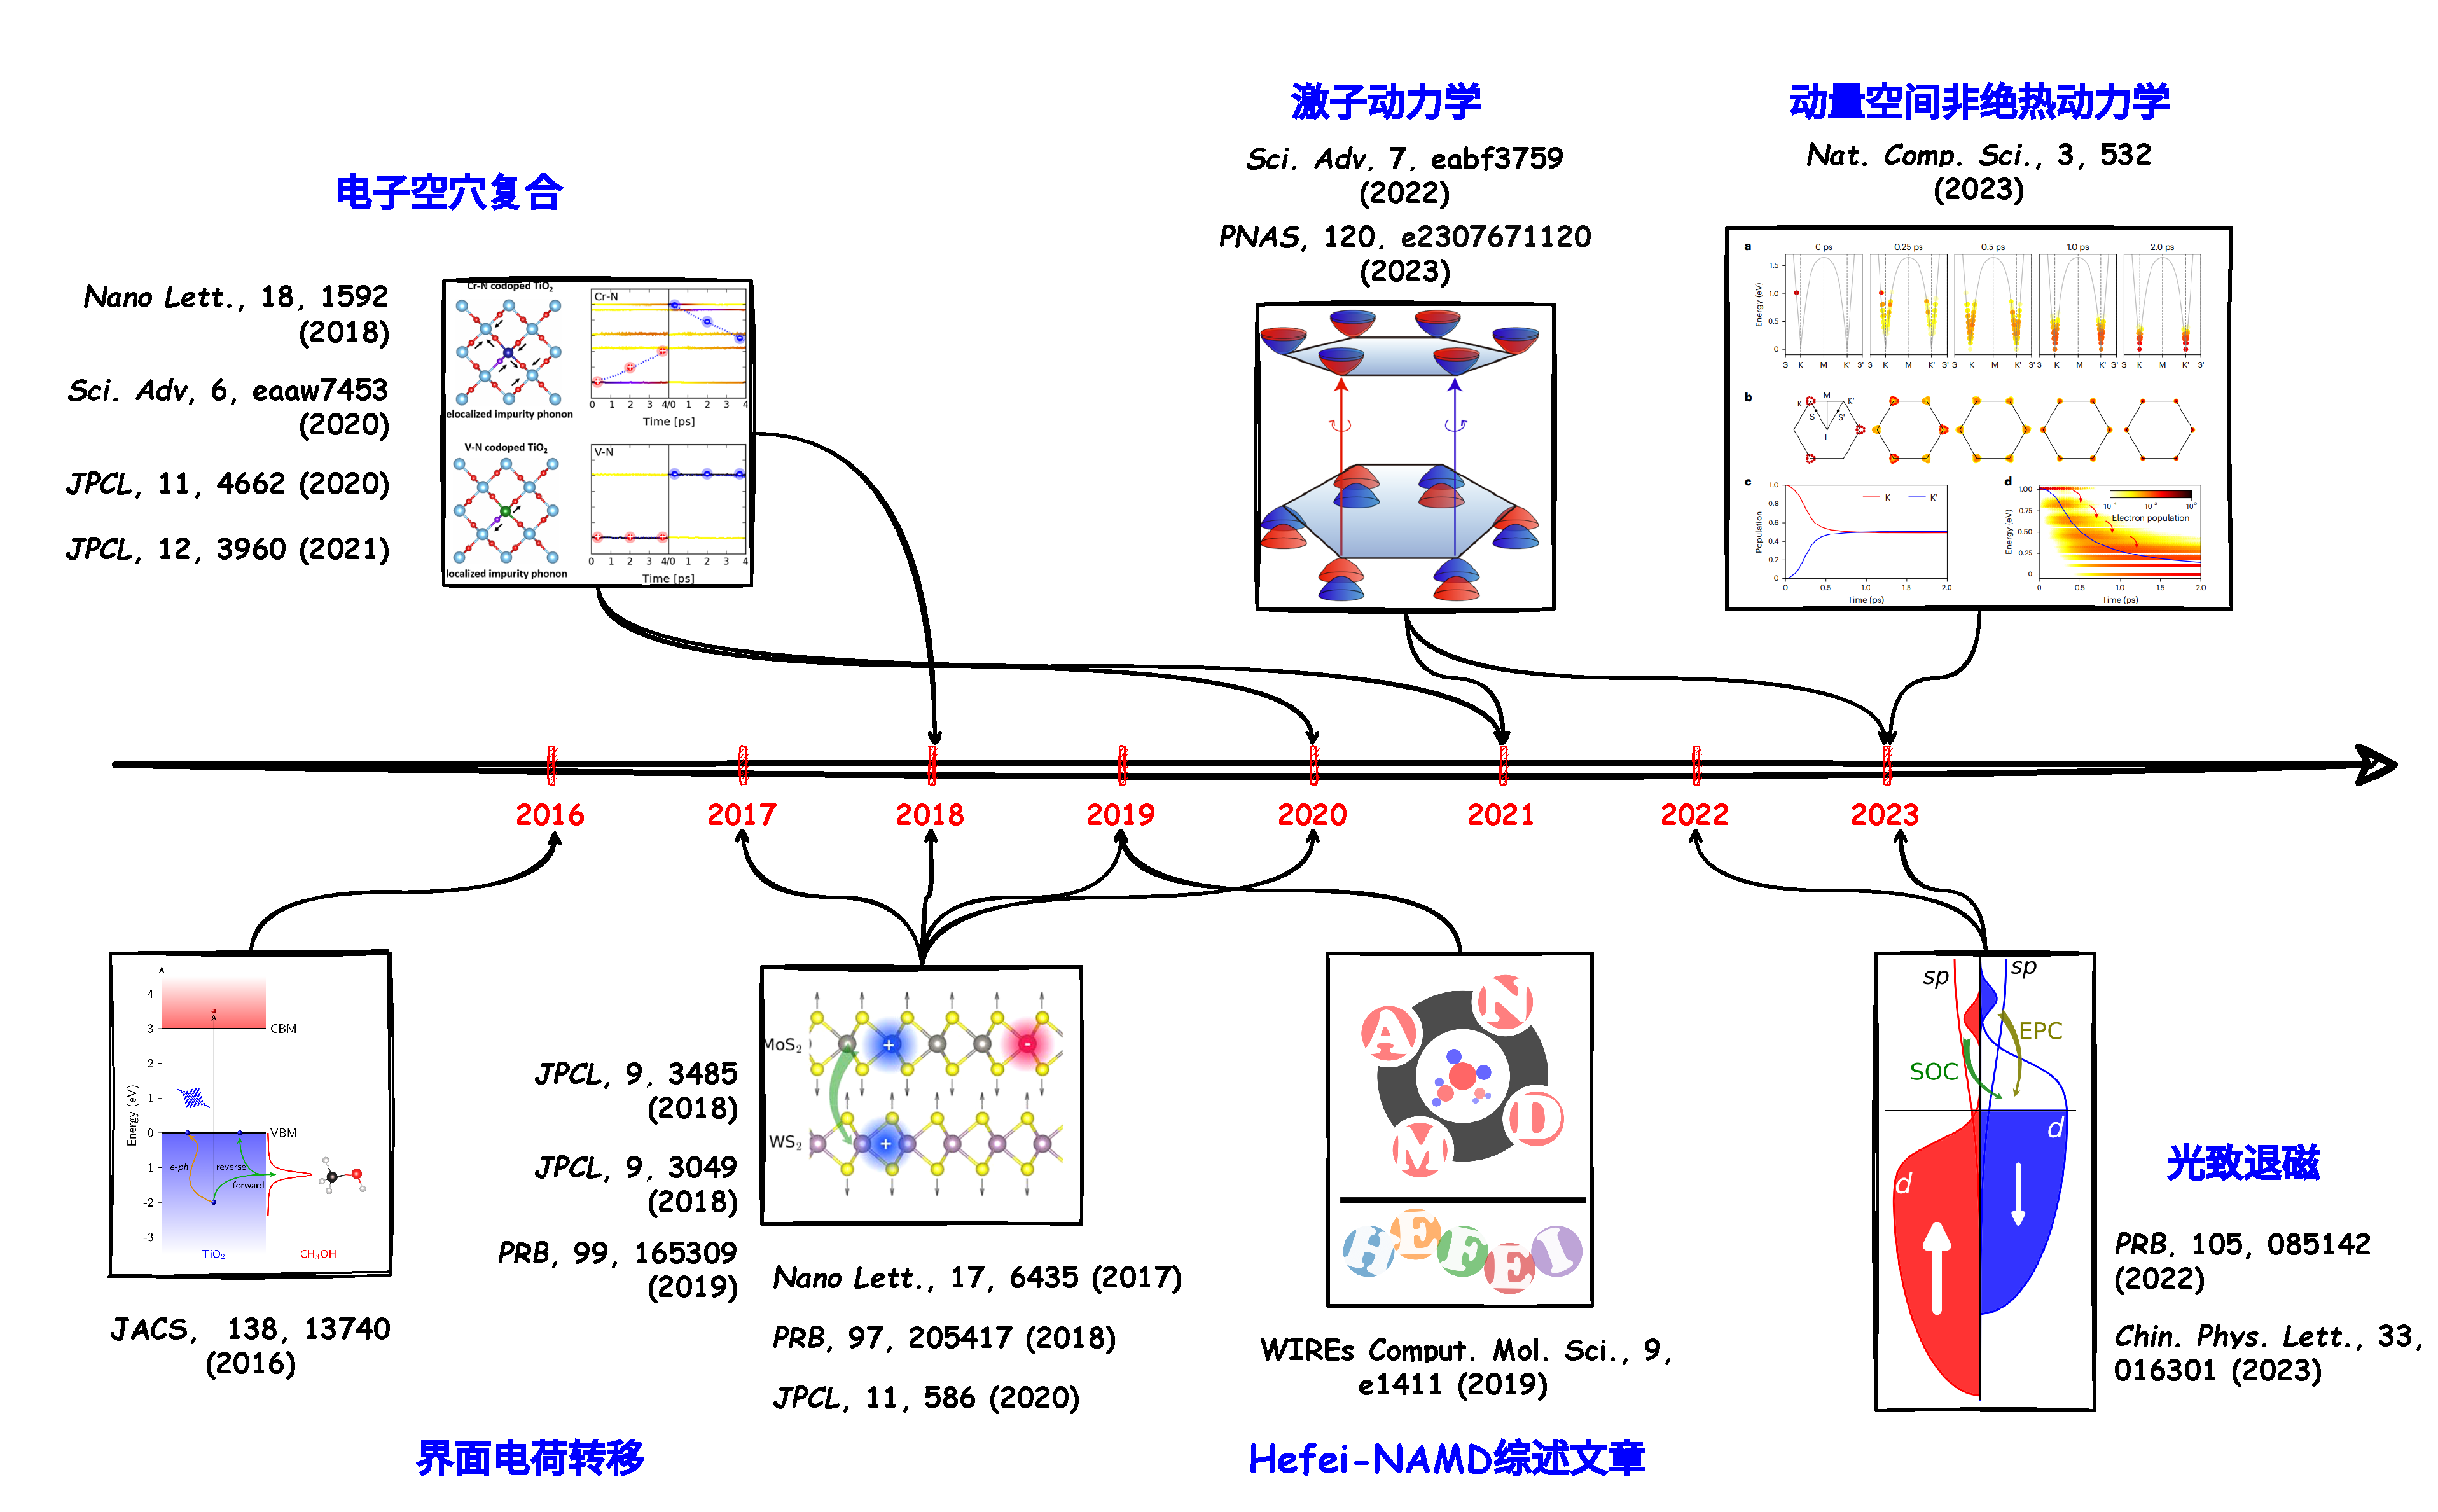
\includegraphics[width=1.\linewidth]{figs/rep_work.pdf}
  \caption{\label{fig:fig_rep_work}
    \kaishu{}
    申请人历年利用Hefei-NAMD做出的一些重要工作总结。
  }
\end{figure}


固体材料中的激发态载流子动力学是影响光电及能源器件效率的关键之一。在太阳能电池、
光电器件、表面等离激元以及光催化等领域,激发态载流子的动力学行为决定了材料与器件
的效率,理解了激发态动力学行为,才有可能解决能源材料与器件领域的重要问题。申请人
分别在界面电荷转移、表面分子激发态以及半导体电子空穴复合三个方向取得了一系列成就,
如图\ref{fig:fig_rep_work}所示。

\begin{enumerate}[label=\textnormal{\color{EmphColor}\Roman*.}]
\item {\color{EmphColor}\kaishu\bfseries{}
    提出范德华异质结、金属纳米颗粒/半导体超快界面电荷转移物理机制
}

  在二维材料兴起之后,范德华异质结材料由于其在光电器件领域的潜力受到了人们大量的
  关注,这类界面相互作用很弱,不存在化学键,但多个实验组都证明界面存在时间尺度在
  数十飞秒的超快电荷转移,这其中的物理机制人们还无法理解。我们利用 \hnamd{} 研究
  了过渡金属硫族化物(TMD)界面的电荷转移过程,发现电声耦合在界面电荷转移中起到了
  非常重要的作用,在 MoS$_2$/WS$_2$ 界面,光学支声子的辅助是空穴超快转移的重要原
  因[\textit{Nano Lett.} 17, 6435 (2017)](代表性工作 2,引
  用 70次),在 MoSe$_2$/WSe$_2$ 界面,由于更强的电声耦合,甚至会发生声子耦合的界
  面电荷振荡[\textit{Phys.\ Rev.\ B}, 97, 205417 (2018)]。我们还进一步提出可以通
  过施加应力的方法调控界面电荷转移的时间尺度[\textit{J.\ Phys.\ Chem.\ Lett.},
  11, 586 (2020)];这些工作成功地揭示了声子激发以及电声耦合在界面电荷转移动力学中
  的重要作用。

  \begin{justify} \kaishu\color{magenta}{}
      % \setlength{\leftskip}{10pt}
      % \setlength{\rightskip}{10pt}

    我们提出的声子辅助电荷转移的机制被哥伦比亚大学 Howard Family 教授 X.Y.  Zhu
    的时间分辨超快实验证实,他们直接观察到了电荷转移与声子的耦合[\textit{Phys.\
      Rev.\ B}, 101, 201405 (2020)], 声子辅助超快电荷转移这一概念也被广泛接受,德
    国巴伐利亚科学院院士 U.  H\"ofer 教授[\textit{Phys. Rev. B}, 102,
    125417(2020), \textit{Nanoscale}, 5, 1603 (2020)],德国马普所
    的 Gierz 教授[\textit{Sci. Adv.}, 6, eaay0761 (2020)], 及浙江大学的朱海明教
    授[\textit{J. Phys. Chem. Lett.}, 10, 150 (2019)] 用我们提出的概念成功地解释
    了他们的实验结果(附录 2.1-2.5)。2019 年被 Web of Science 评为诺奖热门人选的
    斯坦福大学Tony Heinz 教授在其发表在\textit{Nat. Nanotech.}上的综述中评价
    到:“最近一些工作证实了声子在电荷转移中的直接作用\ldots{}人们认为声子可以将电
    子从K谷散射搞$\Gamma$谷,此时层间有更强的杂化,有助于电荷转移的发
    生\ldots{}Zheng等人利用TDDFT方法证实了这个原理。”[\textit{Nat.\ Nanotech.},
    57, 5320 (2018)](附录2.6)。
  \end{justify}

  
\item {\color{EmphColor}\kaishu\bfseries{}
    发现电子空穴复合中心的产生与半导体硬度的关系,提出调控载流子寿命的理论方案
  }

  半导体材料常有的缺陷和杂质会产生电子空穴复合中心,降低器件的效率,如何通过材料
  设计尽量减少半导体材料的电子空穴复合中心是这个领域的重要问题。我们研究了一系列
  半导体材料中的电子空穴复合动力学,在 TiO$_2$ 为代表的氧化物半导体中,我们发现能
  量位于能隙中间的深杂质能级会成为电子空穴复合中心,这与人们熟悉
  的 Shockley-Reed-Hall (SRH) 模型给出的结论一致[\textit{Nano Lett.}, 18, 1592,
  (2018)]。然而,在有机钙钛矿太阳能电池(MAPbI$_3$)的工作中,我们却发现无论是深
  能级缺陷还是浅能级缺陷,都没有形成明显的电子空穴复合中心,分析表明主要原因是由
  于这种材料硬度很低,因此导带底、价带顶与缺陷能级都只与低频声子耦合,从而使得无
  论缺陷是深能级还是浅能级,电子空穴复合都很慢,不会有复合中心的形成。因此,我们
  提出硬度较低的半导体材料不易形成电子空穴复合中心,这类材料可能在清洁能源及光电
  器件方面有重要的应用 [\textit{Sci. Adv.}, 6, eaaw7453, (2020)]上。

  \begin{justify} \kaishu\color{magenta}{}

    文章发表后引起了业内同行的关注,苏黎世理工大学的 KovalenKo 教授用我们提出的概
    念解释了他们的 NMR 和 NQR 实验(JACS 2020)北京师范大学的方维海院士在他们的文
    章中用详细介绍了我们在电子空穴复合方面的工作 (JMCA 2020): “Zhao 与合作者研究
    了不同材料中的电子空穴复合动力学,包括钙钛矿、金红石TiO$_2$、黑磷等,为设计高
    效光伏和光催化材料提供了重要的理论依据\ldots{}”[附录 5.1-5.2]
  \end{justify} 
  
\end{enumerate}
